\chapter{Perzeption und Prädiktion}
\label{chap:perzeption_praediktion}

\section{Sensorik}
\label{sec:sensorik}


\subsection{Registrierung von Farb- und Tiefendaten}

\begin{figure}[htbp]
	\centering
	\begin{subfigure}[t]{0.31\textwidth}
		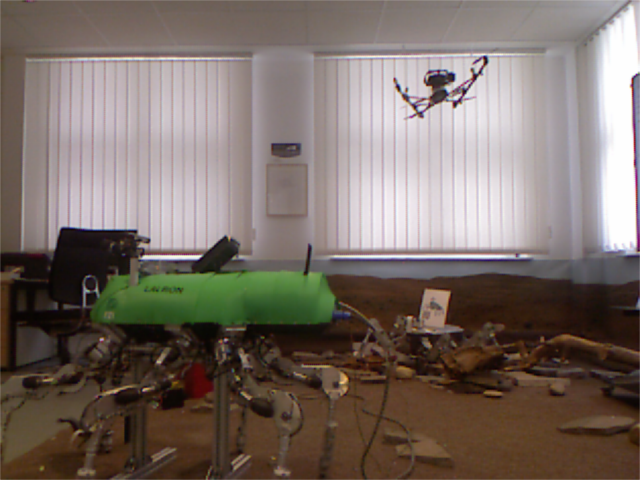
\includegraphics[width=\textwidth]{04_images/motion_prediction/rgbd_example_rgb}
		\subcaption{RGB-Bild}
	\end{subfigure}
	\begin{subfigure}[t]{0.31\textwidth}
		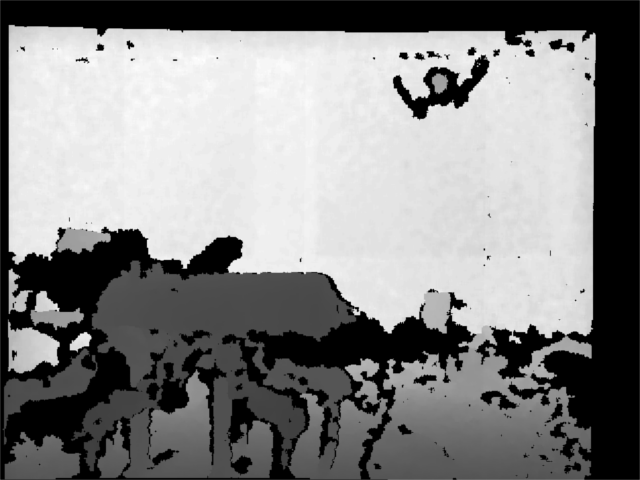
\includegraphics[width=\textwidth]{04_images/motion_prediction/rgbd_example_depth}
		\subcaption{Registriertes Tiefenbild}
	\end{subfigure}
	\begin{subfigure}[t]{0.31\textwidth}
		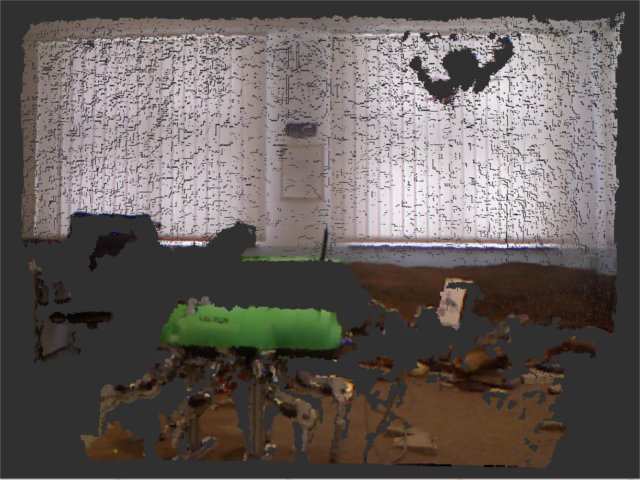
\includegraphics[width=\textwidth]{04_images/motion_prediction/rgbd_example_cloud}
		\subcaption{Eingefärbte Punktwolke}
	\end{subfigure}
	
	\caption[Beispiel der Komponenten einer RGBD-Aufnahme]{Beispiel der Komponenten einer RGBD-Aufnahme aus \citestudthesis{mauch15}. Die 3D-Struktur der Flugdrohne ist in der gegebene Distanz nicht mehr aufzulösen. Schwarz dargestellte Pixel repräsentieren Stellen, an denen keine Tiefenwerte vorliegen. In der gewählten Darstellungsperspektive (die nicht der Kamera-Perspektive entspricht) sind die Abschattungen, 
		welche aufgrund der 2,5D-Datenstruktur entstehen, deutlich sichtbar.}
	\label{fig:rgbd_component_example}
\end{figure}

